\chapter{Grundlagen} \label{CapterFundamentals}

Dieses Kapitel gibt einen Überblick über die in dieser Arbeit verwendeten Terminologien und führt Grundlagen zu Technologien und Techniken ein, welche die Basis für diese, Arbeit bilden. 

Nach der Definition von Augmented Reality werden unterschiedliche Ansätze für die Objekterkennung und -erfolgung vorgestellt.  
Diese sind ein essenzieller Bestandteil der Augmented-Reality-Technologie. Es wird die Definition von Situated Visualization erläutert 
und unterschiedliche Darstellungsformen für die Visualisierung von Daten im Kontext zur physischen Welt (z. B. Gegenstände, Person, Aufgabe) nahe gebracht. 
Abschließend wird die Begriffsdefinition von Usability erläutert und ein Einblick in Usability Engineering gegeben, welches eine etablierte Vorgehensweise für die 
Gestaltung und Entwicklung von Systemen mit hohen Usability Anforderungen ist. 

\section{Augmented Reality}

%Definition und Begriffseingrenzung  von AR
Augmented Reality (zu dt. Erweiterte Realität, kurz \gls{ar}) steht für die Überlagerung der realen Welt mit digitalen Informationen. \cite{Azuma1997,DieterSchmalstieg2016} Im Gegensatz zur Virtual Reality (z. dt. Virtuelle Realität, kurz VR), wo Benutzer vollständig in virtuelle Umgebungen eintauchen,
ist das Ziel von AR, Informationen direkt in die physische Umgebung des Benutzers einzufügen. So soll der Eindruck entstehen, dass diese Informationen Teil der realen Welt sind. \footnote{Nach Definition von Azuma  müssen Informationen hierbei nicht nur auf visuelle Informationen beschränkt sein, 
sondern können auch auditive, haptische, gustative (Geschmack) oder auch olfaktorische (Geruch) Informationen umfassen.} \cite{Azuma1997} Während in VR (kurz für Virtual Reality, dt. Virtuelle Realität) Benutzer von der äußeren Umgebung nichts mitbekommen, wird in AR die reale Umgebung des Benutzers mit virtuellen 
Objekten überlagert. Azuma beschreibt in \cite{Azuma1997}, folgende Charakteristiken für Augmented Reality: 

\begin{enumerate}
	\item Kombiniert reale und virtuelle Welt (Combines real and virtual).
	\item Ermöglicht Interaktionen in Echtzeit. (Interactive in real time)
	\item Informationen (reale und virtuelle) haben einen Bezug im dreidimensionalen Raum. (Registered in 3-D)
\end{enumerate}

Diese Charakteristiken helfen dabei Augmented Reality besser zu verstehen und technologisch einzuordnen. \cite{Azuma1997} Filme, wie z. B. ``Jurassic Park``, in welchem virtuelle Objekte in die reale Szene eingefügt werden, erwecken zwar den Eindruck, dass diese Objekte Teil der realen Szene sind, jedoch kann mit diesen Objekten nicht in Echtzeit interagiert werden. \cite{Tonnis2010} In Filmen werden die virtuellen Objekte in eine zuvor aufgezeichnete Aufnahme eingefügt. 
In der AR Technologie hingegen werden virtuelle Objekte live in ein Video eingefügt. Dies bedeutet, dass in  Filmen für das Einfügen von digitalen Informationen in die reale Szene, eine beliebig große Zeitspanne zur Verfügung steht. 
In AR muss dies in wenigen Millisekunden geschehen. Die neue Position und Ausrichtung des virtuellen Objektes in die live Szene muss innerhalb einer Zeitspanne von zwei Frames bestimmt werden.

Ein anderes Beispiel für AR ist in Live-Ansichten von Digitalkameras zu finden, welche das aufzunehmende Bild als Vorschau anzeigen. Oft blenden diese Informationen zu den aktuellen Einstellungen der Kamera sowie den 
Ladezustand der Batterie im Vorschaubild ein (Siehe Abbildung \ref{img:ar_camera_example}). Diese Informationen überlagern zwar die reale Szene, haben jedoch keinen Bezug zum dreidimensionalen Raum. 
Der elektronische Sucher hingegen, welcher, Objekte (z. B. Gesichter) erkennt und in einem virtuellen Rahmen einrahmt, hat einen Bezug zu den Objekten im 3D Raum. 
Zudem sind Interaktionen in Echtzeit möglich. Bewegt sich das vom virtuellen Rahmen eingerahmte reale Objekt oder die Kamera selbst, verändert sich auch die Position des virtuellen Objektes. 

\begin{figure}
	\centering
	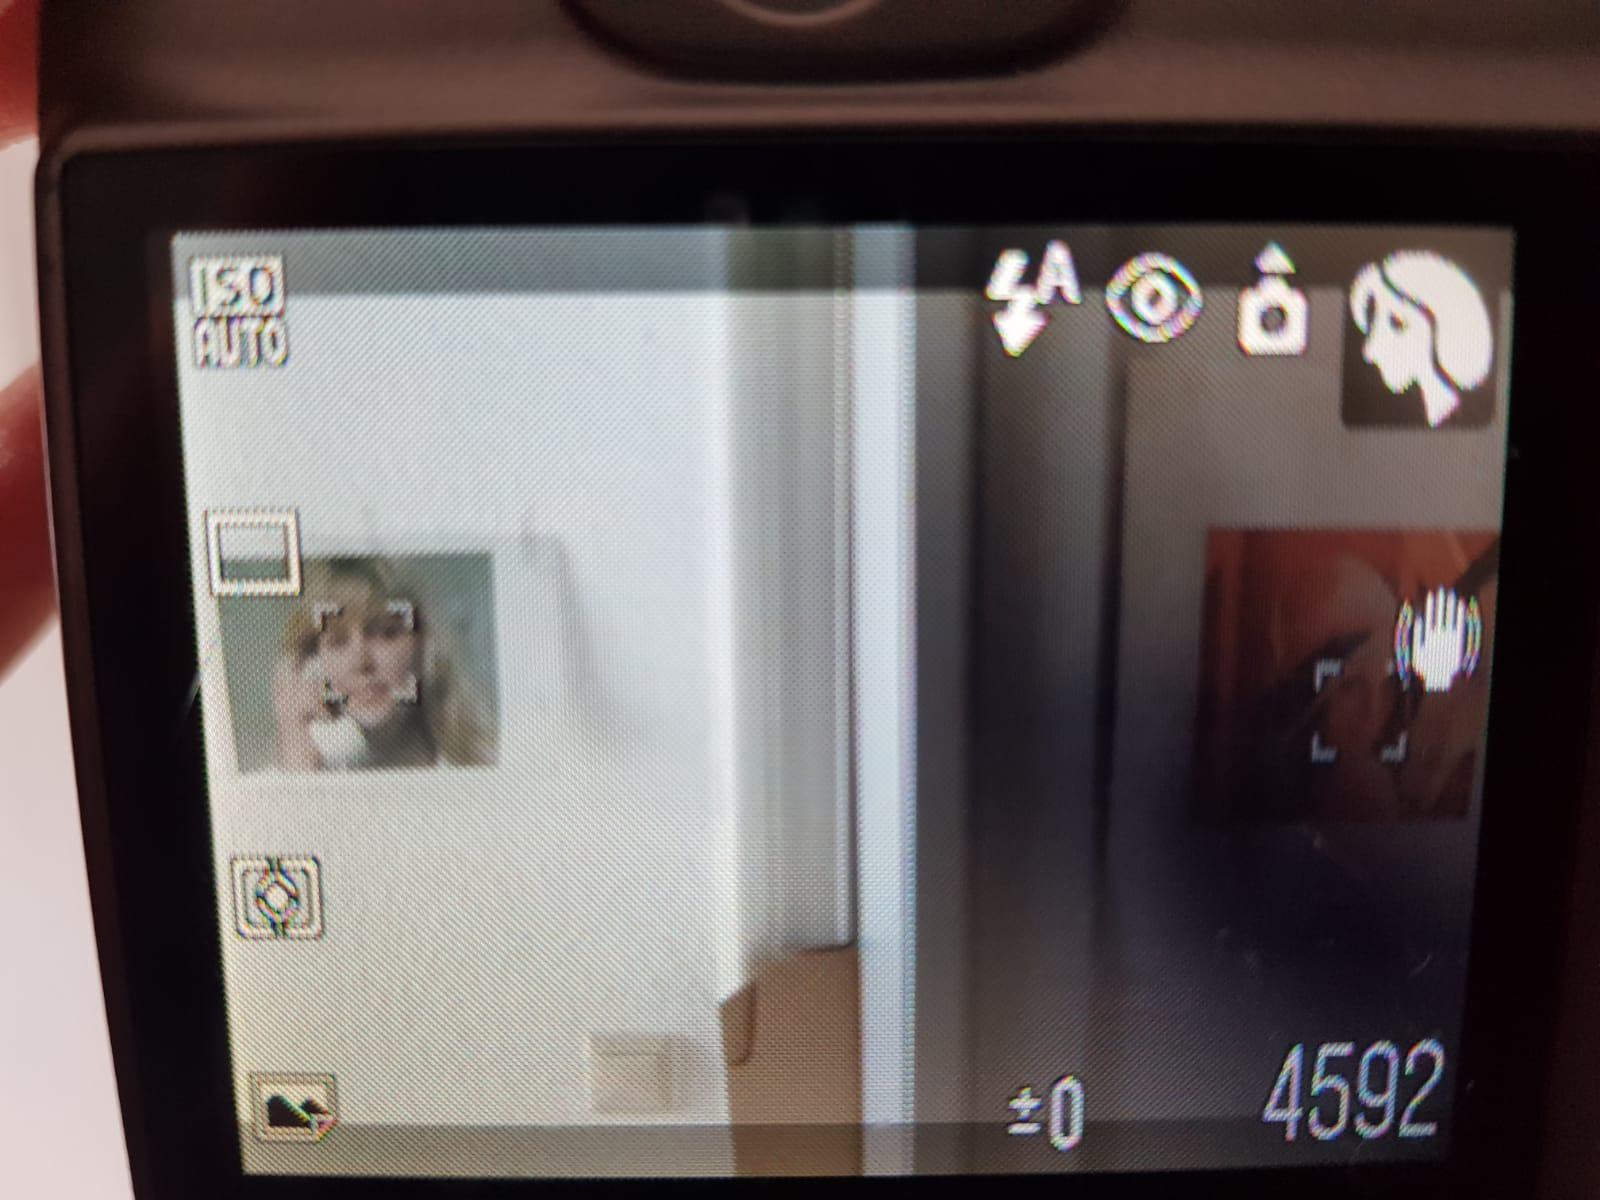
\includegraphics[width=0.50\textwidth]{resources/fundamentals/example_camera_screen_ar}
	\caption{Beispielhafte Darstellung eines Digitalkamera-Display mit eingeblendeten digitalen zusätzlichen Informationen. Quelle: Eigene Darstellung}
	\label{img:ar_camera_example}
\end{figure}

% Motivation
\cite{Azuma1997} Durch das Kombinieren von virtueller und physischer Welt erweitert Augmented Reality die Wahrnehmung des Menschen. Die Motivation von AR ist, dem Menschen durch das Einfügen
von digitalen Informationen in die physische Welt Hinweise zu geben und Details zu zeigen, die er sonst nicht unmittelbar wahrnehmbar wären. Diese Informationen sollen den Menschen 
bei der Verrichtung ihrer Aufgaben in der physischen Welt unterstützen.

% Anwendungsfelder von AR % Besonders passend für diese Arbeit sind Annotationen und Warung und Reperatur. Da diese sich besonders mit Interaktionen an Realen Objekten, meist Produkte befassen.
Azuma fasst in \cite{Azuma1997} Forschungen zu AR in sechs Anwendungsgebiete zusammen: Zur Visualisierung von Medizindaten, in der Wartung 
und Instandsetzung, Annotationen, für die Wegfindung in der Robotik und für die Navigation von Militärflugzeugen. Beispielsweise können Annotationen 
verwendet werden, um Informationen über den Inhalt von Regalen einzublenden, während ein Nutzer durch eine Bibliothek läuft und nach bestimmten Büchern sucht. % Füge hier vielleicht noch ein Beispiel dazu ein % Füge hier Verweis auf ein Artike als Fußnotel hinzu
Auch können Annotationen in AR verwendet werden, um einzelne Bauelemente an komplexen Bauteilteilen zu identifizieren und Informationen über diese zu visualisieren. 
In der Wartung und Instandsetzung können Augmented Reality Anwendungen dabei helfen, Instruktionen an komplexen Maschinen und Anlagen zu visualisieren, welche sonst in 
Form von Text und Bildern vorliegen. So können beispielsweise virtuelle Replikate über die physischen Modelle gelegt und, Schritt für Schritt Anleitungen direkt am physischen Produkt visualisiert werden. 
Durch Animationen können diese Anleitungen präziser gestaltet werden und zum Beispiel auch Informationen über die Richtung geben. 

Diese Systeme können heute zum Beispiel Unternehmen dabei helfen, besser mit ihren Kunden zu kooperieren. In Kombination mit der Technologie Internet of Things (IOT) können Unternehmen
zustands-bezogene Informationen zu Ihren Systemen bei Endkunden abrufen und proaktiv ihre Kunden auf notwendige Wartungen am physischen System aufmerksam machen. Wartungsanleitungen können dann direkt 
an den Anlagen angezeigt werden, sodass Endkunden diese selbständig durchführen können.\footnote{Fallstudie zur Anwendung von AR in Wartung von Industrieanlagen: https://www.ptc.com/-/media/Files/PDFs/Case-Studies/Howden-vuforia-studio-case-study-Feb-2019.pdf?la=en\&hash=6342841E1B6470C1F313295427398606 [letzter Zugriff: 25.06.2019]}

%Grundlegende Techniken
\cite[S.~32]{Tonnis2010} Für die Überlagerung der realen Welt mit virtuellen Objekten eignen sich nach heutigem Stand der Technik zwei Display Techniken, nämlich Optical See-Through und Video See-Through. 
Bei Optical See-Through kann der Nutzer direkt in die reale Welt blicken, wobei computergenerierte Bilder auf einen halbdurchlässigen Spiegel eingeblendet werden (dieses wird als Combiner bezeichnet).
Diese Technik hat den Vorteil, dass der Nutzer einen direkten Blick auf die reale Welt hat. Der Nachteil ist jedoch, dass die reale Welt nicht zeitgleich mit virtuellen Objekten überlagert werden kann. 
Dadurch, dass die Berechnung der Positionsbestimmung und das Rendern der virtuellen Objekte Zeit in Anspruch nimmt, werden diese mit einer kleinen Verzögerung angezeigt. Dies kann, auch 
wenn es sich nur um einige Millisekunden handelt, zu einem so genannten Schwimmeffekt führen (en. Lag). Mit der See Through Display Technik wird die reale Welt dem Nutzer als ein Video 
angezeigt und mit virtuellen Objekten überlagert. Der Vorteil dieser Technik liegt darin, dass die Darstellung der realen Welt um die Zeit verzögert werden kann, die benötigt wird, um die virtuellen Objekte 
richtig zu positionieren und zu rendern. Dadurch werden die Nachteile der Optical-See-Through Technik kompensiert. Dass die reale Welt dem Nutzer verzögert angezeigt wird, bringt jedoch den Nachteil mit sich, 
dass Positionsänderungen physischen, sich in der physischen, sich in der realen Welt befindenden Objekten oder die Änderung der Perspektive, falls sich der Nutzer selbst bewegt, verzögert angezeigt werden. Zudem wird mit 
dieser Technik, je nach Auflösung der Kamera die reale Welt, mit verringerter Qualität angezeigt.

\section{Objekterkennung und -verfolgung}

% Definition von Objekterkennung und Verfolgung
\cite[S.~85]{DieterSchmalstieg2016}Objekterkennung und- Verfolgung beschreibt den Vorgang für die kontinuierliche Bestimmung der Lage und Ausrichtung einer Entität im drei dimensionalen Raum. 
Entitäten können hierbei der Kopf des Nutzers, Augen, ein AR Gerät wie z. B. die Kamera oder ein physisches Objekt in der Umgebung des Nutzers sein. 
Im folgenden werden drei Begriffe erläutert welche oft im Zusammenhang mit Objekterkennung und Verfolgung verwendet werden:
 
\textit{Kallibrierung (engl. Calibration):} Der Vorgang für den Vergleich von Messungen zweier Sensor Geräten wie z. B. eine Kamera. Wobei die Messungen eines Sensors einen Richtwert darstellen gegen die, die
Messungen eines anderen (zu kalibrierenden) Gerätes überprüft und angepasst werden. Durch die Kalibrierung werden Parameter bestimmt durch welche Messwerte des zu kalibrierenden Gerätes einer bekannten 
Maßstab (en. Scale) angepasst werden. 

\textit{Verfolgung (engl. Tracking)}: Beschreibt die kontinuierliche Abtastung bzw. Messung der Umgebung. Dies wird benötigt für die dynamische Registrierung von Objekten im drei dimensionalen Raum. 

\textit{Registrierung (engl. Registration:)} Anpassung der Koordinatensysteme der virtuellen und realen Objekte. Für die Schaffung eines gemeinsamen Koordinatensystems wird die Kalibrierung des AR Systems 
ausgeführt. Dieser Vorgang wird als statische Registrierung bezeichnet (engl. Static registration) und geschieht zu einem Zeitpunkt wo sich der Nutzer bzw. die Kamera nicht bewegt. Bewegt sich der 
Nutzer bzw. die Kamera wird dynamisches Tracking eingesetzt. 

Abbildung \ref{img:komponentsoftracking} veranschaulicht das Zusammenwirken dieser drei Komponente:

\begin{figure}[H]
	\centering
	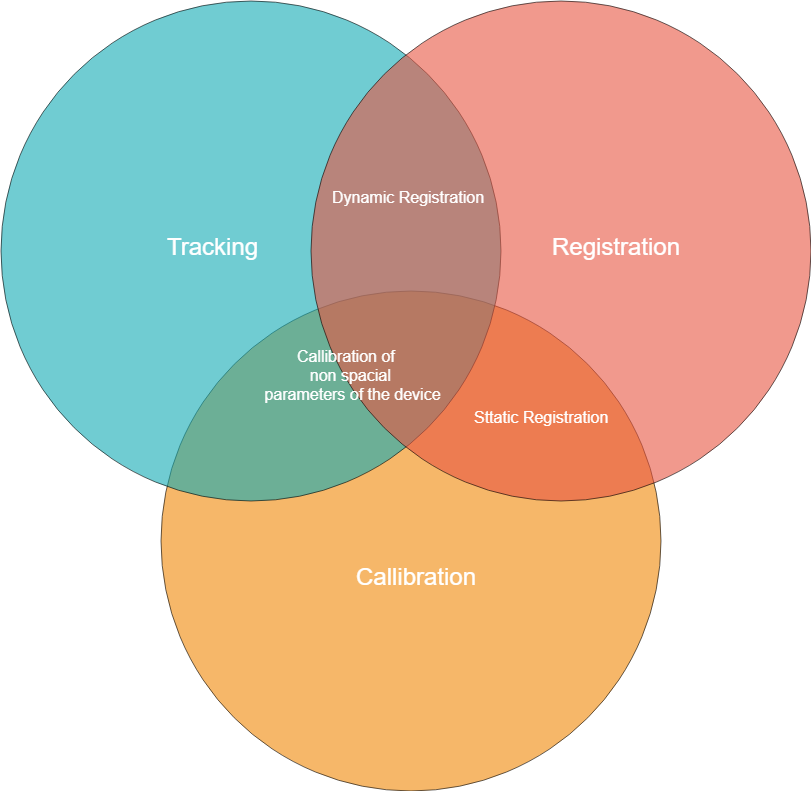
\includegraphics[width=0.4\textwidth]{resources/fundamentals/Tracking.png}
	\caption{Komponente für Objekterkennung und Verfolgung in AR Quelle: In Anlehnung an \cite[S.~86]{DieterSchmalstieg2016}}
	\label{img:komponentsoftracking}
\end{figure}

In AR wird für das Tracking der Umgebung unterschiedliche Sensoren verwendet. Dabei wird zwischen nicht visuellen Sensoren sowie visuellen bzw. optischen Sensoren  unterschieden. 

\textit{Nicht visuelle Sensoren:}  

\textit{GPS (kurz für Global Positioning System):} Mit GPS wird die Positionsbestimmung ermittelt indem Signale an mehrere Satelliten übertragen werden. Die Position des mobilen Endgerätes durch Trilateration zu berechnen ist 
möglich wenn Signale von vier oder mehr Satelliten deren aktuelle Postion im Erdumlaufbahn bekannt sind empfangen werden. Die Genauigkeit dieser Messung variiert stark zwischen 1m bis 100m je nach Anzahl verfügbarer Satelliten. 
\cite[S.~2]{Arora2017}\cite[S.~100]{DieterSchmalstieg2016}Diese Messmethode eignet sich für Positionsbestimmung in Innenräumen nicht besonders gut, da Signale an den Wänden reflektiert werden. 
Höhere Genauigkeit kann mit  DGPS ( kuzr für Differential Global Positioning System) erzielt werden. Die Messwerte werden durch die zusätzliche Übertragung eines Signales welches Korrekturwerte beinhalten, von den Satelliten an eine Basisstation auf der Erde verbessert. \\

\textit{Drahtlose Netze:}\cite[S.~101]{DieterSchmalstieg2016} Netzwerkinfrastrukturen wie WLAN (kurz für Wireless Local Area Network), Bluetooth und Beacons sowie Signale von Mobilfunksendemasten können genutzt werden um die Position des mobilen Endgerätes zu bestimmen. 
Da GPS, WLAN sowie Mobilfunk auf mobilen Endgeräten in der Regel zur gleichen Zeit verfügbar sind, werden meist Informationen dieser drei Sensoren kombiniert eingesetzt um die Abdeckung, Geschwindigkeit sowie die
Genauigkeit der Positionsbestimmung zu verbessern. 

\textit{Magnetometer:}\cite[S.~102]{DieterSchmalstieg2016} Mit dem Magnetometer wird die Ausrichtung des mobilen Endgerätes relativ zum magnetischen Norden ermittelt. 

\textit{Gyroskop: } Der Gyroskop liefert Informationen über die Rotation des mobilen Endgerätes. 

\textit{Beschleunigungsmesser (engl. Linear Accelerometer)}:\cite[S.~104]{DieterSchmalstieg2016} Mit Hilfe des Accelerometer kann relativ zu einer Ausgangsposition die aktuelle Position ermittelt werden. Zudem kann in Kombination mit einem Magnetometer
die Rotation sowie die Position ermittelt werden. 

\textit{Optische\ Visuelle Sensoren:}\\

Zu den visuellen Sensoren in mobilen Endgeräten zählt die Kamera. Dieses liefert Bildinformationen. Nach aktuellem Stand der Technik besitzen einige Smartphones auch bereits Kameras welche Informationen über die Tiefe liefern. Diese Informationen werden in Computer Vision Algorithmen für das Tracking und das Registrieren von virtuellen Objekten in die reale Welt genutzt. Mit mobilen Endgeräten wird eine Kombination aus nicht visuellen und visuellen Sensoren verwendet um ein optimales Tracking zu ermöglichen.

% Oft wird eine Kombination von nicht visuellen sowie visuellen Sensoren eingesetzt um optimale Ergebnisse zu erzielen. 

Die optischen Trackingverfahren unterteilen sich in \textit{Modellbasierte} und \textit{Modellfreies} Trackingverfahren unterteilen. 

Bei Modellbasierten Trackingverfahren wird vor dem Tracking für die Registrierung, ein Modell festgelegt welches erkannt werden soll um virtuelle Objekte relativ zum festgelegten Modell zu platzieren. 
Hierbei kann ein Modell ein Marker oder ein Bild mit einzigartigen Bildmerkmalen aus der natürlichen Umgebung des Nutzers (engl. Natural Features) sein. 

Marker sind für das Tracking erstellte (quadratische oder kreisförmige) Bilder oder Barcodes. Diese sind mit besonders ausfälligen und kontrastreichen Mustern gestaltet. Alternativ zu Markern können Bilder aus der natürlichen Umgebung des Nutzers verwendet werden.\cite{Cukovic2015} Bei diesen Verfahren werden Algorithmen verwendet wie zum Beispiel SIFT \footnote{Scale-invariant feature transform}, SURF \footnote{(Scale Invariant Feature Transform} oder Ferns um einzigartige Bildmerkmale aus Video während dem Tracking und dem vorher festgelegten Bild zu vergleichen.

Neben Bilder können bei modellbasierten Trackingverfahren auch dreidimensionale CAD Modelle von physischen Objekten verwendet werden. \cite{Lowney2016} Wie auf Abbildung \ref{img:modellbased_categories} zu sehen ist, lassen sich Methoden für das Tracking von 3D Modellen in zwei Kategorien unterteilen. In rekursives Tracking sowie in Tracking by Detection. Bei Recursiven Tracking Verfahren wird die vorherige Pose \footnote{Position und Ausrichtung des Modells} genutzt um die neue Pose abzuschätzen. Tracking bei Detection Verfahren sind in der Lage die neue Pose des Modells zu berechnen, ohne die vorherige Pose zu kennen. Aufgrund ihrer ihre rekursiven 
Funktionsweise benötigen Recursive Tracking Methoden jedoch weniger Rechenleistung als Tracking by Detection Methoden. 

\begin{figure}[H]
	\centering
	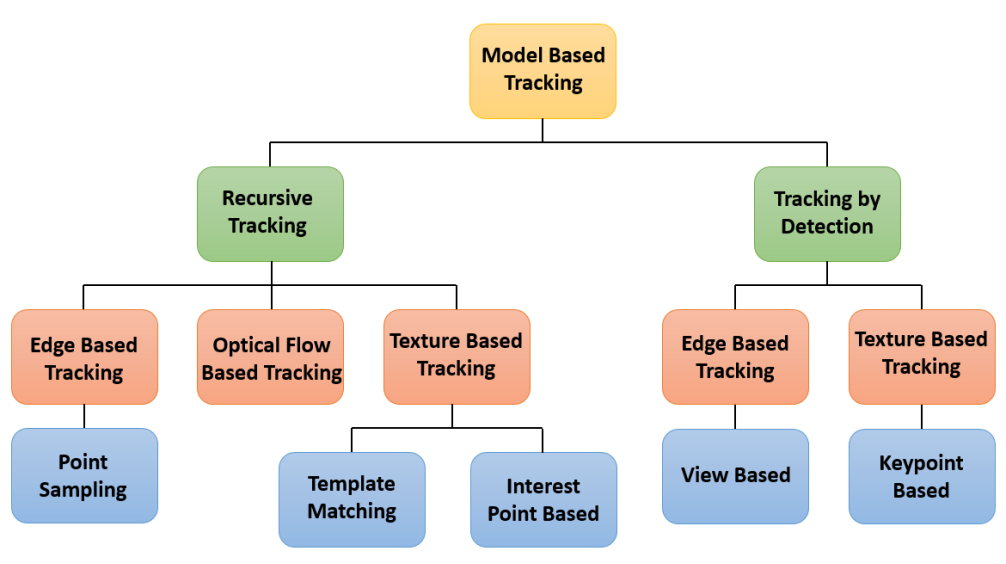
\includegraphics[width=0.6\textwidth]{resources/fundamentals/model_based_tracking_taxonomies.png}
	\caption{Kategorien der modellbasierten Tracking Verfahren mit Verwendung von CAD Modellen. Quelle: \cite[S.~86]{Lowney2016}}
	\label{img:modellbased_categories}
\end{figure} 

Modellfreie Tracking Methoden benötigen keine vorher festgelegten Modelle zum platzieren der virtuellen Objekte in die reale Umgebung. \cite[S.~106]{DieterSchmalstieg2016} Das Modell wird während dem Trackingvorgang 
erstellt. Dadurch dass im Voraus kein Modell für das Tracking erstellt werden muss, sind modellfreie Trackingmethoden flexibler in der Nutzung. Da die Modelle ausgehend vom Startpunkt während dem Trackinvorgang 
erstellt werden, kann die zu realen Objekten in der Umgebung relative Ausrichtung der virtuelle Objekte nur spontan (zur Laufzeit) bestimmt werden. 

Mit einigen Frameworks können modellfreie wie modellbasierte Verfahren kombiniert werden. So kann mit einer modellbasierten Verfahren die Ausrichtung der virtuellen Objekte, relativ zu einer vorher festgelegten Modell festgelegt werden. Mithilfe von modellfreies Tracking kann das Tracking aufrecht erhalten werden auch wenn die Kamera, das Modell welches für das modellbasierte Verfahren festgelegt wurde, nicht oder nur teilweise im Sichtfeld hat. 

Zu den modellfreien Methoden zählt das PTAM Verfahren (kurz für  Parallel Tracking and Mapping), welches an das aus der Robotik stammende Verfahren SLAM (kurz für Simultaneous Localization and Mapping) angelent ist. \cite{Klein2007} Mit PTAM wird während des Trackings eine Karte der Umgebung des Nutzers aus einzigartigen Bildpunkten erstellt. Bei diesem Verfahren werden zwei sepearte Threads \footnote{Leichtgewichtiges Prozess womit Programmteile parallel oder pseudoparallel nebenläufig ausgeführt werden können.} eingesetzt. Ein Thread übernimmt die Aufgabe des Trackings. Dieser läuft wird schnell ausgeführt (mit z. B. 30 Hz). Ein zweiter Thread wird für für das Mapping eingesetzt. Dieser wird langsamer ausgeführt und ist mit dem Tracking Thread über sogenannte Keyframes verbunden. Keyframes sind Bilder aus dem Video. Neue Keyframes werden aufgenommen wenn sich das aktuelle Videobild stark von den vorhandenen Keyframes unterscheidet. Ein weiter Kriterium für die Aufnahme eines neuen Keyrames ist, dass dieses eine bestimmte Qualität vorweisen muss (z. B. nicht durch zu starke Bewegung verschwommen ist). Diese Methode eignet sich besonders gut für natürliche bzw. schnelle Kamerabewegungen.

\begin{figure}[H]
	\centering
	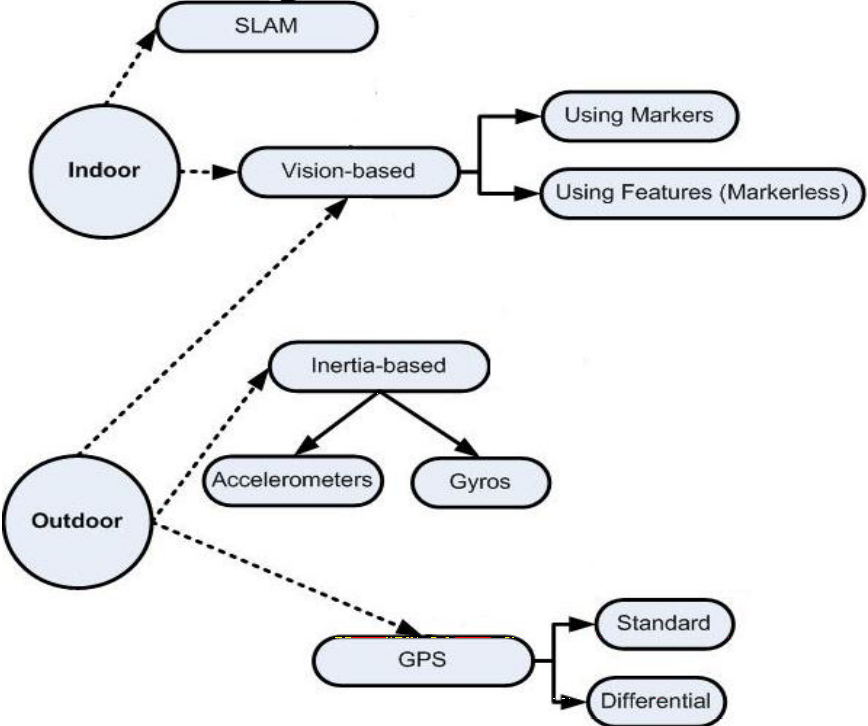
\includegraphics[width=0.4\textwidth]{resources/fundamentals/tracking_technicken.png}
	\caption{Überblick unterschiedlicher Trackingverfahren für Innen und Außenbereiche. Quelle: \cite{Arora2017}}
	\label{img:overviewTrackingMethods}
\end{figure}

Abbildung \ref{img:overviewTrackingMethods} zeigt ein Überblick über Trackingverfahren und macht eine grobe Einordnung für die Eignung hinsichtlich Innen und Außenbereichen.

\section{Situated Visualization}
\subsection{Situated Visualization - Definition}


Das zu konzipierende System soll durch den Einsatz von Augmented Reality die Abgabe von Feedbacks zu Produkten und deren Darstellung auf den Produkten bzw. Produktteilen ermöglichen. 
Als eine besondere Form von Visualisierung beschäftigt sich das Feld Situated Visualization mit der Visualisierung von Daten im Kontext zu physischen Objekten. 

\cite[S.~239]{DieterSchmalstieg2016} Ein großer Vorteil von Augmented Reality Nutzeroberflächen ist deren Fähigkeit, Situation, Aufgaben oder Nutzer-relevante Informationen in 
der realen Umgebung des Nutzers anzeigen zu können. Diesen Vorteil zunutze zu machen ist jedoch stark davon abhängig, welche Informationen in welcher Form in AR dargestellt werden.
Situated Visualization befasst sich mit der richtigen Präsentation von computergenerierten
Grafiken von physischen Gegenständen oder Personen in der realen Szene. \cite[S.~188]{Marriott2018} Die Bedeutungsbestimmung wird durch die Kombination von Visualisierung und deren 
Beziehung zu der unmittelbaren Umgebung erreicht. \cite[S.~240]{DieterSchmalstieg2016} Abzugrenzen von Situated Visualization sind Visualisierungen, welche zwar im 3D Raum präsentiert werden, jedoch keinen Bezug zu einem im dreidimensionalen Raum befindlichen Objekt, Person oder Aufgabe haben.

\cite[S.~192]{Marriott2018} \cite[S.~2]{Willett2017} stellen das in Abbildung \ref{img:situated_visualization_concept} dargestellte konzeptionelle Modell 
zur Situated Visualization vor.

\begin{figure}[H]
	\centering
	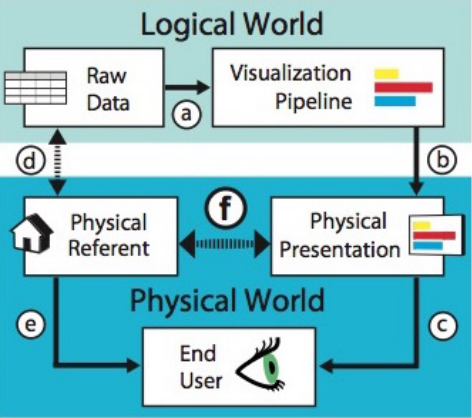
\includegraphics[width=0.5\textwidth]{resources/fundamentals/situated_visualization/spacially_situated_visualization_model.png}
	\caption{Konzeptionelles Model zu Situated Visualization. Quelle: \cite[S.~192]{Marriott2018}}
	\label{img:situated_visualization_concept}
\end{figure}

% spacially situated visualization
Dieses Modell (siehe Abbildung \ref{img:situated_visualization_concept}) erweitert die konventionelle Visualisierung der logischen Welt (Abbildung \ref{img:situated_visualization_concept} oberer Abschnitt) um die der physischen Welt (Abbildung \ref{img:situated_visualization_concept} unterer Abschnitt). 
Die durchgängig dargestellten Pfeile (Abbildung \ref{img:situated_visualization_concept} (a), (b), (c) und (e)) zeigen den Informationsfluss zwischen den einzelnen Komponenten, die gestichelten Pfeile (Abbildung \ref{img:situated_visualization_concept} (d) und (f)) die konzeptionellen Beziehungen. Der Informationsfluss beginnt bei den Rohdaten in der oberen linken Ecke der Darstellung. Die Rohdaten durchlaufen die \gls{visualisierungspipeline} und werden in eine vom Menschen besser interpretierbare visuelle Form umgewandelt (Abbildung \ref{img:situated_visualization_concept} (Abbildung \ref{img:situated_visualization_concept} a $\rightarrow$ b)). Die Verbindung zwischen logischer und physischer Welt wird mithilfe zweier Beziehungen hergestellt (b und d). 
Die physische Präsentation der Daten (Abbildung \ref{img:situated_visualization_concept} (b)) stellt die Präsentation der Daten in visueller Form in der realen Welt dar. 
Dies könnte zum Beispiel eine Visualisierung in Form einer Annotation sein, welche der Betrachter durch eine Datenbrille auf einem physischen Gegenstand sieht. Es könnte eine Auflistung von Daten, welches 
auf dem  Display eines Smartphones oder Tablet angezeigt wird oder ein Preisschild, welches in ausgedruckter Form an einen physisches Gegenstand angebracht ist.

Die zweite Beziehung besteht zwischen Rohdaten und physischen Referenten. Diese Beziehung ist ein Konzept, da Datensätze sich auf mehrere unterschiedliche Referenten beziehen können. 
Der Grad, inwieweit der physische Referent und die physische Präsentation gleichzeitig wahrgenommen werden können, hängt von der räumlichen Distanz zwischen diesen beiden ab (Abbildung \ref{img:situated_visualization_concept} (f)). 

Der Betrachter könnte die Daten mithilfe von Augmented Reality auf dem physischen Referenten betrachten. Der Betrachter könnte vor dem physischen Referenten stehen und die Daten zu dem Referenten auf
dem Bildschirm seines Smartphones betrachten. Der Betrachter könnte aber auch räumlich entfernt vom physischen Referenten sein, sodass er diesen nicht sehen kann und die Daten auf einem Ausgabegerät 
wie einem Computerbildschirm betrachten. 

%Physically- vs. Perceptually-Situated Visualizations 
\cite[S.~194]{Marriott2018} Da Distanzen jedoch relativ zu Größe von Objekten wahrgenommen werden, kann die physische und die wahrgenommene Distanz zwischen dem Physischen Referenten und der Physischen Präsentation stark voneinander abweichen. Wenn beide Objekte zum Beispiel nur wenige cm groß sind, kann ein Abstand von einem Meter sehr groß erscheinen, während der gleich Abstand für ein sehr großes Objekt, wie zum Beispiel ein Berg in einer Landschaftsansicht, zum Beispiel sehr klein erscheint. 

%Zeitlich distanz (temporal)
\cite{Willett2017} Neben der räumlichen Distanz muss auch die zeitliche Distanz zwischen dem aktuellen Zustand des Physischen Referenten und die der physischen Präsentation hinsichtlich dessen 
Aktualität betrachtet werden. 
Die zeitliche Distanz ist die zeitliche Abweichung zwischen den Daten die dem aktuellen Zustand des physischen Referenten entspricht, und den Daten welche in der Physischen Präsentation visualisiert werden.
Werden beispielsweise Temperaturwerte die ein Temperatursensor an einem physischen Objekt anzeigt betrachtet und es wird der aktuell gemessene Wert angezeigt gibt es keine zeitliche Distanz. Wird jedoch ein
historischer Wert angezeigt oder eine Vorhersage, kann die zeitliche Distanz stark variieren.

%embedded visualisierung
\begin{figure}[H]
	\centering
	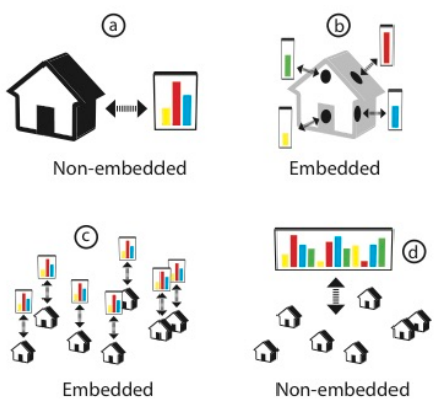
\includegraphics[width=0.5\textwidth]{resources/fundamentals/situated_visualization/embedded_visualization.png}
	\caption{Embedded und Nicht-Embedded Situated Visualisierungen. \cite[S.~195]{Marriott2018}}
	\label{img:embedded_visualization}
\end{figure}

\cite[S.~195]{Marriott2018} Embedded Visualization stellen eine besondere Art von Situated Visualization dar, welche sehr stark in die physische Umgebung integriert sind. 

Abbildung \ref{img:embedded_visualization} zeigt eingebettete und nicht eingebettete (Situated) Visualisierungen. \cite[S.~202]{Marriott2018} Ist ein Objekt aus mehreren Einzelteilen 
zusammengesetzt und die Daten zu den Einzelteilen, werden in einer Visualisierung in der Nähe des Objektes dargestellt, gilt die Visualisierung als Situated, jedoch nicht als Embedded (Abbildung \ref{img:embedded_visualization} (a)).
Werden die Daten zu den Einzelteilen, jeweils in der unmittelbaren Nähe der jeweiligen Einzelteilen dargestellt, gilt die Visualisierung als Embedded (Abbildung \ref{img:embedded_visualization} (b)). Ist ein, Einzelteil jedoch nur einmal in einem Produkt vorhanden (zum Beispiel ein Motor in einem Auto), gilt die Visualisierung zu diesem Einzelteil nicht als Embedded. 

Embedded Visualization geht davon aus, dass mehrere Teil-Visualisierungen zu den jeweiligen physischen Referenten entsprechen. Befinden sich in einem Haus beispielsweise mehrere Steckdosen und der Stromverbrauch 
für jede Steckdose wird jeweils in der unmittelbaren Nähe der jeweiligen Steckdose visualisiert, gilt die Visualisierung als Embedded. Gibt es in dem Haus jedoch nur eine Steckdose, gilt die Visualisierung nicht mehr als
Embedded.

\vspace{15mm} 
\begin{figure}[H]
	\centering
	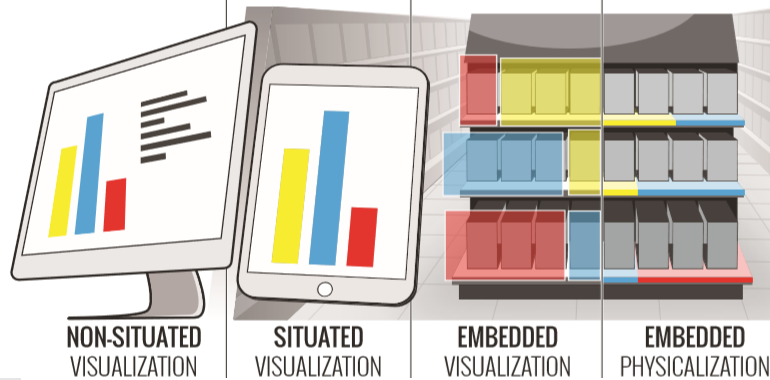
\includegraphics[width=0.5\textwidth]{resources/fundamentals/situated_visualization/Illustration_situated_embedded_visualization.png}
	\caption{Illustration mit unterschiedlichen Visualisierungen am Beispiel von Produkten in einem Supermarkt-Regal}
	\label{img:Illustration_situated_embedded_visualization}
\end{figure}

Mit Hilfe der Illustration in Abbildung \ref{img:Illustration_situated_embedded_visualization} zeigen \cite{Willett2017} am Beispiel von Produkten, 
welche in einem Supermarkt in einem Regalen platziert sind, die Eigenschaften unterschiedlicher Visualisierungen und die damit verbundenen Vor- und Nachteile der jeweiligen Visualisierungsform. 

Der Vorteil von Non-Situated Visualisierungen (Abbildung \ref{img:Illustration_situated_embedded_visualization} ganz links) ist, dass diese flexibler hinsichtlich Standort 
der Nutzung und Hardwareanforderungen gestaltet werden können. Der Betrachter kann sich in dieser Form der Visualisierung räumlich getrennt von den Produkten befinden und die Visualisierung 
auf einem beliebigen Display wie zum Beispiel einem Computerbildschirm, auf dem Display eines Smartphones oder Tablett ansehen. Der Nachteil dieser Art der Visualisierung ist jedoch dass kein 
direkter Bezug zwischen den angezeigten Informationen und den physischen Produkten bzw. Produktteilen hergestellt werden kann. 

Am Beispiel von (Abbildung \ref{img:Illustration_situated_embedded_visualization} ganz links), wäre dem Betrachter, ohne die Unterstützung einer Beschreibung der Lage wo sich die Produkte im 
Supermarkt befinden oder mit Hilfe einer Karte, nicht möglich, eine Beziehung zwischen der, physischen Platzierung der Produkte im Verkaufsraum und deren Umsatz herzustellen.

Situated Visualization ermöglicht dem Betrachter, Produkte bzw. Produktteile und Visualisierungen zu diesen, zur gleichen Zeit betrachten zu können. Dies bring den Vorteil dass eine Beziehung 
zwischen Lage und Ausrichtung der Produkte bzw. Produktteile und den visualisierten Informationen hergestellt werden kann. Diese Form der Visualisierung erfordert jedoch, dass sich 
der Betrachter räumlich nahe am Produkt befindet und die Visualisierung auf einem mobilen Endgerät anzeigt wird.

Embedded Visualization ermöglichen dem Betrachter, die Visualisierung der Daten unmittelbar an den jeweiligen Produkten bzw. Produktteilen zu betrachten ohne den Blick von diesen abwenden zu müssen. 
Dies bringt den Vorteil dass der Betrachter während er die Visualisierung betrachtet, seinen Blick nicht vom Produkt bzw. Produktteil abwenden muss und Informationen zur direkten Umgebung des Produktes bzw. Produktteiles wahrnehmen kann. Diese Form der Visualisierung erfordert dass sich der Betrachter vor den entsprechenden Produktteilen befindet und Ausgabetechniken verwendet werden, welche die Informationen unmittelbar in der Nähe der 
Produktteile anzeigen (z. B. mit AR).

Am Beispiel von (Abbildung \ref{img:Illustration_situated_embedded_visualization} zweite von rechts) wird dem Betrachter ermöglicht, Informationen zur unmittelbaren Umgebung der Produkte (zum Beispiel eine zu schwache Beleuchtung, einen unangenehm riechenden Geruch, ein Windzug, usw.) wahrzunehmen, während er die Visualisierung (welches ihm zum Beispiel zeigen könnte dass der Umsatz für diese Produkte während der vergangenen Monate zurück gegangen ist) zu diesen Produkten unmittelbar an den Produkten betrachtet.  

%Facsimiles
\cite{Willett2017}Eine Möglichkeit, um Daten im Kontext zu physischen Objekten zu visualisieren, ist auch über die Verwendung von so genannten Faksimiles möglich. Diese sind detailgetreue, skalierbare Nachbildungen von Objekten, oder eine Instanz eines Objektes, welche durch eine Klasse oder ein Modell klar definiert ist. Ein Faksimile wird für gewöhnlich verwendet, falls die Visualisierung am echten physischen Referenten schwierig bis unmöglich ist. Dies ist der Fall, wenn die physischen Referenten: Sehr klein (z.Bsp. Atome), sehr groß (z Bsp. ein Flussverlauf) zu weit entfernt (z. Bsp: auf einem anderen Planeten) oder sehr fragil bzw. wertvoll sind (z. B. ein Gemälde). 
In solchen Begebenheiten kann die Nutzung von Faksimiles die räumliche Distanz zum betrachtenden Objekt reduzieren und es damit zugänglicher machen. Ein Faksimile kann wenn diese mit ausreichender detailgetreue nachgebildet ist wie der eigentlichen physische Referent betrachtet werden. Die Nutzung von Faksimiles verringert jedoch, die Möglichkeit für den Betrachter, den eigentlichen Referenten zu verändern oder wichtige Details zu betrachten. Dies kann durch den Einsatz von Telepräsenz \footnote{Telepräsenz ist eine Form von Videokonferenz und beschreibt die Möglichkeit, virtuell an entfernten Orten Präsent zu sein. Siehe: https://www.itwissen.info/Telepraesenz-telepresence.html [Zuletzt aufgerufen am: 28.06.2018]} kompensiert werden. 


\subsection{Situated Visualization - Techniken und Herausforderungen}

Im folgenden Abschnitt wird ein Überblick über die Herausforderungen für die Darstellung von Daten im Kontext zu realen Objekten 
gegeben und Techniken für die Bewältigung dieser Herausforderungen vorgestellt.

\cite{DieterSchmalstieg2016} Bei der Darstellung von Informationen im Kontext zu realen Objekten stellen sich folgende Herausforderungen:

\begin{itemize}
	\item Überladene Darstellung (Unübersichtlichkeit)
	\item Fehler in der Registrierung (Objekterkennung und Verfolgung)
	\item Visuelle Interferenzen
\end{itemize}

\textbf{Überladene Darstellung (Unübersichtlichkeit):}

\cite[S.~241]{DieterSchmalstieg2016} Situated Visualization steht vor den gleichen Herausforderungen welche auch bei traditionellen Visualisierungen auftreten. 
\textbf{Überladene Darstellung (Unübersichtlichkeit)}: 'Wird eine große Menge an Informationen dargestellt, kann dies dies schnell zu einer überladenen Darstellung führen, welches dem Betrachter, einen Einblick 
über die dargestellten Daten zu gewinnen erschwert. Da die Darstellung der Daten in AR Anwendungen, auf die Fläche der real existierenden Objekte begrenzt ist, 
wird diese Herausforderung besonders verschärft. Es eignen sich hierfür zwei Lösungsansätze: Die Datenmenge kann durch Filterung der Daten reduziert werden. 
Dafür kann das ``Information seeking mantra`` von Shneiderman \cite{Shneiderman1996} angewendet werden. 
Bei diesem Konzeopt, wird dem Nutzer zunächst ein Überblick über die gesamte Datenmenge gegeben. Dem Nutzer wird die Möglichkeit gegeben, in bestimmte Bereiche der Daten hineinzuzoomen, Teile der Daten 
welche nicht von Interesse sind auszublenden und einige Teile der Daten auszuwählen zu welchen mehr Details angezeigt werden sollen. 

Beispielsweise kann dies in AR Anwendungen angewendet werden in welcher Annotationen zu Objekten aus der realen Welt visualisiert werden. 
Abbildung (\ref{img:annotation_clutter}) zeigt ein Beispiel in welcher dem Nutzer, Informationen zu Bücher in einer Bibliothek al Annotationen angezeigt werden. Auf (Abbildung \ref{img:annotation_clutter} links) werden 
alle Annotationen zu Büchern welche der Suche des Nutzers entsprechen dargestellt. (Abbildung \ref{img:annotation_clutter} rechts) werden Annotationen zu Bücher mit ähnlichen Eigenschaften gruppiert dargestellt. 
Der Nutzer kann auf eine Gruppe klicken um die Annotationen welche in einer Gruppen zusammengefasst dargestellt sind, zu entfalten. 

\begin{figure}[H]
	\centering
	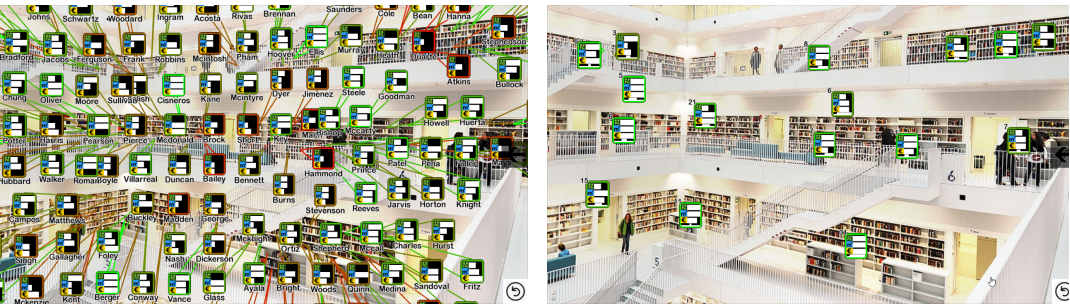
\includegraphics[width=1.0\textwidth]{resources/fundamentals/annotations_clutter.png}
	\caption{Annotationen zu Büchern in einer Bibliothek. Quelle: \cite[S.~1]{Tatzgern2016}}
	\label{img:annotation_clutter}
\end{figure}

Werden virtuelle Darstellungen nahe an realen Objekten platziert, können diese wichtige Details aus der realen Welt sowie andere virtuelle Informationen verdecken. 
Verschiedene Arbeiten beschäftigen sich mit der Behandlung von Verdeckung (\cite{Grasset2012}, \cite{Bell2001}).

In dieser Arbeit wird das Problem der Überladenen Darstellung, bei der Implementierung des Prototypen nur dahingehend behandelt dass der Vorgang für die Erstellung von 
Feedbacks durch die Darstellung vorhandener Feedbacks auf dem Produkt nicht beeinträchtigt wird. 

% data overload wird nicht in der implementierung des prototypen behandelt, muss jedoch unbedingt für die Gestaltung und Konzeption des Gesamtsystems beachtet werden. 
\textbf{Fehler in der Objekterkennung und Verfolgung:} Visualisierungen in AR müssen einen Bezug zu der Objekten aus der realen Umgebung herstellen. Fehler
in der Objekterkennung und Verfolgungen führen zur ungenauen Ausrichtung der Visualisierung.% \cite[S.~88]{Tonnis2010} Auch wenn sich 

Dies erfordert die Einführung von Fehlerbehandlung. \cite[S.~243]{DieterSchmalstieg2016} Um dem Nutzer zum Beispiel zu ermöglichen die den Kontext Darstellung trotz einer fehlerhaften 
Registrierung zu verstehen, können die Umrisse des Referenzen dargestellt werden.

\begin{figure}[H]
	\centering
	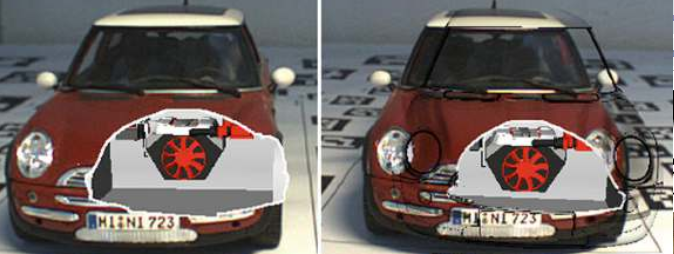
\includegraphics[width=0.7\textwidth]{resources/fundamentals/missallignement.png}
	\caption{Links: Durch die Fehlerhafte Registrierung wird der virtuelle Inhalt falsch platziert. Rechts: Durch die zusätzliche Darstellung der Umrisse des Objektes wird der Kontext wieder richtig hergestellt. Quelle: \cite[S.~243]{DieterSchmalstieg2016}}
	\label{img:missallignement}
\end{figure}

SDKs bieten die Möglichkeit, Informationen zum aktuellen Zustand der Objekterkennung abzurufen (z. B. ob das Objekt aus der realen Welt gefunden wurde und die Objektverfolgung im Gange ist, ob das Objekt verloren wurde und daher nicht weiter verfolgt werden kann, ob zu wenig Bildmerkmale gefunden werden und die Objekterkennung bald verloren gehen kann). 
Diese Informationen können genutzt werden um auf Fehler zu reagieren und zum Beispiel dem Nutzer entsprechende Anleitungen zur weiteren Bedienung zu geben.

\textbf{Visuelle Interferenz:}
\cite[S.~243]{DieterSchmalstieg2016} Visualisierungen heben relevante Daten hervor und lenken die Aufmerksamkeit des Nutzers zu diesen Informationen. In Situated Visualization 
wird die Aufmerksamkeit des Nutzers auf relevante Teile aus der realen Welt, der aktuellen Szene gelenkt. Eine Herausforderung dabei stellt, dass irrelevante Aspekte der realen Welt 
keinen störenden Einfluss haben. \cite{Kalkofen2007} stellen Techniken vor Teile aus der realen Umgebung in den Fokus zu rücken während andere den Kontext dazu herstellen. 

In AR stellt sich die Herausforderung, dass Visualisierungen sich auf Änderungen der realen Szene anpassen müssen. Dies kann zum Beispiel die Änderung der Lichtverhältnisse sowie die 
Änderungen des Hintergrundes sein. \cite{Gabbard} Die Änderung des Hintergrundes wie Farbe, Textur, Beleuchtung haben zum Beispiel einen signifikanten Einfluss auf die Lesbarkeit von Texten.   

\section{Computerunterstützte Kollaboration}

Durch die Verwendung des zu entwickelnden Systems, sollen Anwendungsszenarien unterstützt werden, in welchen Nutzer, 
über Feedbacks auf Produkten bzw. Produktteilen kommunizieren können. Diese Kommunikation soll eine Kollaboration von 
mehreren Nutzern, mit dem Produkt im Mittelpunkt zu ermöglichen und zum Ziel haben, die Qualität der Produkte und die 
damit verbundene Kundenzufriedenheit zu verbessern.     

In der computerunterstützten, kooperativen Zusammenarbeit (en. Computer-Supported Cooperative Work (CSCW)) 
ist eine Kategorisierung die Rodden in \cite[S.~2]{Rodden1992} beschreibt, sehr verbreitet.  


Rodden betrachtet bei dieser Kategorisierung zwischen Nutzern zwei Dimensionen der Kommunikation zwischen Nutzern: 
Die räumliche Distanz zwischen Nutzern sowie die zeitliche Differenz im Nachrichtenaustausch, dabei erfolgt einen Unterteilung zwischen 
Remote oder Co-Located und Synchron oder Asynchrone Kommunikation.

Die zeitliche Dimension definiert, ob mehrere Nutzer zur gleichen Zeit (synchron) miteinander kommunizieren 
oder zu unterschiedlichen, also (asynchron/ zeitlich unabhängig voneinander) kommunizieren. Die räumliche Dimension 
gibt Aussage darüber, ob sich die Nutzer während der Kommunikation am gleichen Ort befinden (Co-located) oder räumlich getrennt voneinander sind (Remote). 

\cite[S.~188]{ElSayedNevenA.M.BruceH.ThomasRossT.Smith2015} beschreiben darüber hinaus eine Mischform von Remote und Co-located Kommunikation. 
Bei dieser Form von Kollaboration können eine Teilmenge der Nutzer sich am gleichen Ort befinden, während ein anderer Teil entfernt, 
also (Remote), mittels Telepräsenz an der Kommunikation teilnehmen. 

Schmalstieg und Höllerer \cite[S.~362]{DieterSchmalstieg2016} beschreiben auf Grundlage dieser Unterteilung mögliche 
Anwendungsgebiete für AR Systeme (Siehe Tabelle \ref{tab:categorycscw}).

\cite[S.~362]{DieterSchmalstieg2016} In Co-Located und synchronen Anwendungsszenarien (z. B. eine Besprechung in einem Besprechungsraum), können 
Augmented Reality Anwendungen, die Nutzern dabei unterstützen, Informationen im gemeinsamen Raum zu betrachten zu manipulieren und zu diskutieren. 

In Remote und synchronen Szenarien können AR-Systeme es ermöglichen dass ein Nutzer (Nutzer 1), einem anderen Nutzer (Nutzer 2 welcher räumlich getrennt von Nutzer 1 befindet), 
Informationen über dessen reale Umgebung zu zeigen kann (z. B. Installations- oder Reparatur-Anleitungen). \footnote{Ein AR App der Firma PTC welches Nutzern über eine synchronen Kommunikation, Informationen in die Umgebung des jeweils anderen einzublenden: https://www.ptc.com/de/news/2017/vuforia-chalk [Zuletzt aufgerufen am 21.08.2019]} 

\begin{table}[htbp]
\caption{Kategorisierung Computer unterstützter Kooperationssysteme mit Bezug zu AR. \\Quelle: \cite[S.~362]{DieterSchmalstieg2016}}
	\begin{center}
		\begin{tabular}{|l|ll|}
		\hline
		 & \textbf{Co-located} & \textbf{Remote}\\
		\hline
		\textbf{Synchronous} &  AR shared space & AR telepresence \\
		\textbf{Asynchronus} & AR annotating/ browsing (in-situ) & Generic sharing\\
		\hline
		\end{tabular}
	\end{center}
	\label{tab:categorycscw}
\end{table}

\cite[S.~362]{DieterSchmalstieg2016} Zu den Anwendungsszenarien für asynchrone Kommunikation in AR Anwendungen zählt das Erstellen von Annotationen in der 
physischen Umgebung und das spätere, an Ort und Stelle, Durchforsten und Bearbeiten dieser Annotationen durch andere Nutzer.		

\begin{comment}
Rodden beschreibt in \cite{Rodden1992} 

- Erzeugung von viel breitere Gruppendiskussionen und Aufzeichnung dieser Diskussionen(Report) (z.Bsp. Foren, Community Beiträge).\cite{Rodden1992} cite{Benbunan-Fichet} 
- Gibt Nutzern die Flexibilität, immer dann Beiträge zu erstellen wenn diese Zeit dazu haben.
- Ermöglicht, Nutzern sich mit Teilproblemen befassen für das sie sich am besten befähigt fühlen.
- Zusammensetzung von Informationen aus eine Vielzahl von Quellen und Nutzern


Roden \cite{Rodden1992} ordnet asynchrone Kollaboration zu den Co-Authoring Systemen. Diese sind Systeme, welche mehreren Nutzern, asynchrone Zusammenarbeit 
an einem Artefakt ermöglichen. Jeder Nutzer kann dabei an einem Teil des Dokumentes arbeiten und die Ergebnisse werden zusammengeführt. Asynchrone Kollaboration 
unterstützt laut Rodden einen Grundlegenden Teil von Kooperation, indem es die 
 can produce broader discussions and more complete reports from group discussions than their face-to-face counterparts
 enabling people to contribute whenever they have time to provide input
 they can work on the part of the problem that they feel most qualified to address
 can combine information from a variety of sources

 Co-authoring systems aim to support some of the most fundamental parts of cooperation by supporting the negotiation processes
 for commenting - multiple users working on 
 store and forward and real-time communication systems

notwendigkeit für unterscheidung zwischen private, public oder direkte nachrichten 

[Rodden seite 20]
 [Rodden seite 24] Co-authoring systems aim to support some of the most fundamental parts of cooperation by supporting the negotiation processes % for commenting %multiple users working on % [Rodden seite 24]store and forward and real-time communication systems. %
The general model adopted by these systems is that of asynchronous co-operation with each user working independently on a portion of the document. Reviews and comments are added to the document by annotating sections of the document. 

\end{comment}

\section{Usability}

Nach der Implementierung eines digitalen Prototypen, soll im Rahmen einer Nutzerstudie die Usability (dt. Benutzbarkeit) des Prototypen evaluiert werden.
Daher wird in diesem Abschnitt, die Definition von Usability näher betrachtet. Anschließend wird ein Einblick in Usability Engineering gegeben welches eine etablierte Herangehensweise für
die Gestaltung und Entwicklung von Systemen mit hohen Usability Anforderungen ist. 

\subsection{Usability - Definition} \label{UsaDef}

% Begiffserklärung von Usability
In der Normreihe ISO 9241 welches als ein internationaler Standard, Richtlinien für die Gestaltung von Mensch-Computer-Interaktionen beschreibt, wird im ISO Norm 9241-11,  Usability (zu dt. Benutzbarkeit) wie folgt definiert:

``\textit{Das Ausmaß, in dem ein Produkt durch bestimmte Benutzer in einem bestimmten Nutzungskontext genutzt werden kann um bestimmte Ziele effektiv, effizient und zufriedenstellend zu erreichen.}``

%Die Benutzbarkeit eines Systems muss im Kontext seiner Verwendung beurteilt werden.[Michael Richter, Markus Flückiger]
Dass die Usability eines Systems nach dessen Nutzungskontext zu bewerten ist verdeutlichen \cite[S.~10]{MichaelRichter2016} an einem konkreten Beispiel für die Erfassung 
von Kurznachrichten (SMS) mit dem Aufkommen von Mobiltelefonen. Bevor Smartphones mit Touch-Displays verbreitet waren, hatten Mobiltelefone oft rein numerische Tastaturen sodass, das Erfassen 
von Textnachrichten über die Nutzung der numerischen Tasten erfolgen musste. Indem zum Beispiel in kurzen Zeitabständen zwei mal auf die Taste ``2`` gedrückt wurde, wurde zu Beispiel der Buchstabe 
``B`` eingegeben. Diese Eingabemethode wurde oftmals von vielen Nutzern als umständlich empfunden. Jedoch konnte auf diese Weise effizient und zufriedenstellend die Aufgabe, eine Kurznachricht 
zu erfassen erfüllt werden. Zudem war diese Methode einfach zu erlernen und einprägsam. Somit wies dieser Ansatz für den damaligen Stand der Technik eine hohe Usability auf. 

% Eine Teilmenge der Systemazeptanz 
Nielsen stellt in \cite[S.~25]{Nielsen1994} Akzeptanzkriterien für ein Systeme vor und stellt Usability als eine Teilmenge die dieser Kriterien vor.
Akzeptanzkriterien unterteilt er in soziale und praktische Kriterien.

Soziale bzw. ethische Akzeptanzkriterien sind solche, welche die Nutzer von der Nutzung eines Systems abhalten, auch wenn praktische Akzeptanzkriterien sehr gut erfüllt werden. 

Um die gewünschte Funktionalität zu ermöglichen, werden mit Augmented Reality Anwendungen viele Informationen über die Umgebung des Nutzers erhoben.\cite[S.~3]{Roesner2013} Es wird auf die Kamera, gegebenenfalls auf den Lautsprecher sowie verschiedene Sensoren wie z. B. den Gyroskop, Accelerometer usw. zugegriffen. Dies birgt Risiken dass diese Daten missbräuchlich genutzt, gestohlen und die Privatspähehe von Nutzern verletzt werden können. \cite[S.~9]{Templeman2012} Die Studie PlaceRaider beweist, dass mithilfe von Kamera und Sensordaten eines Smartphones die Umgebung des Nutzers detailliert genug rekonstruiert werden kann, um sensible Informationen wie z. B. Kontodaten auf einem Kontoauszug ablesen zu können. \cite{Roesner2013,Lebeck2018} stellen weitere Risiken für die Beeinträchtigung der Privatsphäre von Nutzern vor welche als soziale Akzeptanzkriterien bei der Gestaltung von Augmented Reality Systemen beachtetet werden sollten. 

Unter den praktischen Kriterien sowie Usability (zu dt. Benutzbarkeit) auf. Die Eigenschaft Benutzbarkeit gliedert er in die Eigenschaften Nützlichkeit (en. Utility) und Gebrauchstauglichkeit (en. Usability) auf. Unter Utility (zu dt. Nützlichkeit) ist zu verstehen ob ein System mit den Funktionalitäten die es bereitstellt in der Lage ist, die Aufgabe zu erfüllen wozu sie konzipiert wurde.

Die Eigenschaft Benutzbarkeit gliedert Nielsen in folgende fünf Teileigenschaften: 

\begin{itemize}
	\item Einfach zu erlernen.
	\item Effizient in der Nutzung.
	\item Leicht zu merken. (Ein Nutzer welcher das System bereits einmal verwendet hat, sollte in der Lage sein nach einer längeren Pause das System nutzen zu können ohne es erneut erlernen zu müssen.)
	\item Wenig Fehler. (Das System sollte während der Nutzung zu möglichst wenig Fehler führen. Im Falle das Fehler auftreten, sollte es möglich sein dass sich das Systems von diesen Fehlern erholt sodass die Nutzung des Systems fortgeführt werden kann.)
	\item Subjektive Zufriedenstellung (Das System sollte angenehm zu nutzen sein. So dass Nutzer auch subjektiv zufriedengestellt werden während sie das System nutzen.)
\end{itemize}

\begin{comment}
%7 Kritärien nach ISO 9241 Teil 110 - ASSEFIL) 
Im ISO Norm  9241-110 sind diese Kriterien, als Grundsätze zur Dialoggestaltung wie folgt aufgeführt:

\begin{itemize}
	\item Aufgabenangemessenheit \footnote{Beispiele für Aufgabenangemessenheit ab Seite 5: https://www.medien.ifi.lmu.de/lehre/ss16/id/ISO\_9241-10.pdf [zuletzt aufgerufen am: 26.06.2019]}
	\item Selbstbeschreibungsfähigkeit
	\item Steuerbarkeit
	\item Erwartungskonformität
	\item Fehlertoleranz
	\item Individualisierbarkeit
	\item Lernförderlichkeit
\end{itemize}
\end{comment}

\subsection{Usability Engineering}\label{UsaEng}

\cite[S.~7]{MichaelRichter2016} Im laufe der Zeit haben sich verschiedene Fachrichtungen (wie z. Bsp: Human Computer Interaction (HCI), Human Factors, Interaction Design, Usability Engineering, 
User centered Design (UCD), User Experience (UX) und Design Thinking) entwickelt welche nutzenorientierte Methoden für die Entwicklung von Technologien und neuen Anwendungen verfolgen. 

% Usablity Engineering
\cite[S.~14]{MaryBethRossonJohnM.CarrollDianeD.Cerra2002} Als eines dieser Fachrichtungen wurde die Fachrichtung Usablity Engineering von Usability Fachleuten bei Equipment Corporation ins Leben gerufen.  
Der Begriff Usability Engineering steht für die Konzeption, die Techniken für die Planung, Verifizierung und Abdeckung von Usability Zielen eines Systems. Das Ziel von Usability Engineering ist, 
messbare Usability Ziele in den frühen Phasen des Softwareentwicklungsprozesses zu definieren und einen Rahmen zu schaffen diese Ziele im laufe der Entwicklung stetig überprüfen zu können 
um sicherstellen zu können dass diese erreicht werden.

Mayhew \cite{Mayhew1999} und Nielsen \cite{Nielsen1994} stellen Prozessmodelle für Usablity Engeneering Projekte vor und benennen diese als ``The Usability Engineering Lifecycle``. Mayhew macht in der von ihr vorgestellten Model eine Unterteilung in drei Phasen welche weitere Schritte beinhalten. Nielsen hingegen gliedert sein Model in elf Schritte. Im folgenden werden fünf 
dieser Schritte, genauer betrachtet: 

\vspace{5mm}
\textbf{Benutzerprofile}\label{userprofile}  
 
\cite[S.~73]{Nielsen1994} In diesem Schritt werden alle Nutzer identifiziert, die mit dem zukünftigem System in Berührung kommen werden. Als Nutzer werden Personen verstanden welche mit dem System oder mit Artefakten die durch das Systems entstehen in Berührung kommen werden. Dies kann Personen beinhalten welche das System installieren, konfigurieren, warten, administrieren sowie Endnutzer des Systems. In einigen Fällen, ist es einfacher potenzielle Nutzer eines neuen  Systems zu identifizieren und deren Charakteristiken zu analysieren. Dies ist der Fall wenn Produkte für eine ganz bestimme Nutzergruppe vorgesehen sind. 
Zum Beispiel für Produkte welche in einer bestimmten Abteilung eines Unternehmens in Einsatz kommen sollen. Schwieriger ist die Analyse von Nutzern hingegen für Produkte welche von einer breiteren Menge von Nutzern genutzt werden sollen. 

Folgende Informationen sollten über die Nutzer erhoben und analysiert werden: Der Erfahrungsstand des Nutzers (z Bsp. in Verwendung von solchen Systemen und Endgeräten), Bildungsstand, Alter des Nutzers, Arbeitsumgebung, Lebensumstände, usw. Dieser Schritt ist wichtig um die Lernfähigkeit von Nutzern besser einschätzen zu können und so Kriterien für die Komplexität der Nutzeroberfläche zu bestimmen.

% task analysis 
\textbf{Aufgabenanalyse}\label{task_anlyse}  

\cite[S.~75]{Nielsen1994} Sobald die Nutzer identifiziert und deren Eigenschaften sowie Bedürfnisse analysiert wurden, werden die Ziele und Aufgaben der Nutzer analysiert. Wie bewältigen die Nutzer aktuell Aufgaben um ihre Ziele zu erreichen? Hierbei sollte beobachtet werden welche Informationen die Nutzer benötigen, welche Ausnahme oder Not Situationen auftreten und wie die Nutzer in diesen Situationen handeln. 
Es sollte beobachtet werden ob die Nutzer das aktuell verwendete System in irgendeiner weise umgehen (engl. Workarounds anwenden). Zudem sollten die im Bezug auf die zu lösende Aufgabe, verwendeten 
Terminologien festgehalten werden. Diese können später als eine Quelle für Metapher bei der Gestaltung der neun Nutzeroberfläche verwendet werden. 

% functional analysis TODO: Füge Referenz mit seitenzahl hinzu
\cite[S.~77]{Nielsen1994} Als nächstes werden in diesem Schritt die benötigten Funktionalitäten des neuen Systems analysiert und Möglichkeiten erforscht wie diese mit dem neuen System erzielt werden können. 
Es ist wichtig dass in diesem Schritt die Mögliche Umsetzung der Funktionalitäten sich nicht ausschließlich an Lösungen von bereits bestehenden Systemen orientiert sondern 
bessere geeignete Umsetzungsmöglichkeiten erkundet werden.

% evolution of the user TODO: Füge Referenz mit seitenzahl hinzu
\cite[S.~78]{Nielsen1994} Zuletzt werden Möglichkeiten erforscht wie sich das Nutzungsverhalten der Nutzer über die Zeit, mit der Nutzung des neuen Systems entwickeln könnte. Dieser Schritt wird  
benötigt um das neue System flexibel genug und offen für neue Anforderungen gestalten zu können. 

\vspace{5mm} 
\textbf{Analyse bestehender Produkte} 
 
\cite[S.~78]{Nielsen1994} In diesem Schritt werden bestehende Produkte mit ähnlichem Aufgabenfeld analysiert. Diese können für die Konzeption des neuen Systems als Prototypen dienen. 
Da bestehende Systeme vollständig umgesetzte Funktionalitäten beinhalten, können diese einfach getestet werden.    
Diese Systeme können heuristisch evaluiert werden, es können Nutzer Studien durchgeführt werden oder es kann eine vergleichende Analyse durchgeführt werden falls mehrere Systeme zur 
Verfügung stehen. Auf Basis der Informationen welche, im Schritt ``Benutzerprofile`` zusammengetragen wurden, wird in diesem Schritt des Usablity Engineering Lifecycle, analysiert wie gut die Funktionalitäten und Interaktionstechniken 
bestehender Systeme die Nutzer bei der Umsetzung ihrer Aufgaben unterstützen. Zusätzlich können technischen Produktrezessionen, hilfreiche Informationen über bestehende Systeme geben. 
Da nicht alle Aufgaben bereits eine Software Lösung existiert, schließt Nielsen die Betrachtung von Lösungen welche nicht aus dem Software bzw. Computer Bereich stammen mit ein. 

\vspace{5mm} 
\textbf{Usability-Ziele festlegen} 

Wie im Abschnitt \ref{UsaDef} beschrieben, setzt sich die Usability eines Systems nicht nur aus einer Eigenschaft zusammen sondern gliedert sich in mehrerer Teileigenschaften wie Erlernbarkeit, Fehlertoleranz usw. \cite[S.~79]{Nielsen1994} Oft ist es nicht möglich alle Usability Kriterien mit gleicher Gewichtung zu priorisieren. In diesem Schritt werden auf Grundlage der erstellten Benutzerprofile sowie der Aufgabenanalyse, Prioritäten für die einzelnen Usability Eigenschaften definiert. 

Dafür werden die Usability Eigenschafen operationalisiert und in messbaren Zielen ausgedrückt. Meistens werden Messintervalle für angestrebte Werte, für minimal zu erreichende Werte und theoretisch optimale Werte definiert. Als minimal zu erreichende Werte sind, gelten der Regel Werte welche aktuell mit dem System erreicht werden kann. Usability Ziele für neue Versionen von bestehenden Systemen oder für Systeme für welche vergleichbare andere Systeme existieren, festzulegen ist deutlich einfacher als für neue Systeme wozu keine Vergleichswerte vorliegen. Ein Vorgehen für solche Systeme ist, einige mit dem System zu lösende Aufgaben zu definieren und mehrere Usability Spezialisten nach realistischen Werten zu fragen welche erzielt werden könnten.

\vspace{5mm} 
\textbf{Prototypen und Szenarien}

\cite[S.~93]{Nielsen1994} Die Implementierung eines Systems sollte nicht auf Basis der Gestaltung von Benutzeroberflächen in den frühen Phasen der Konzeption stattfinden. 
Stattdessen können Prototypen in den frühen Phasen eingesetzt werden. Auf diese weise können, Zeit und kostensparend Prototypen des finalen Systems in den frühen Gestaltungsphasen
evaluiert werden. Prototypen lassen sich in zwei Dimensionen unterteilen (Abbildung \ref{img:ver_hor_protptypes}): 

\begin{figure}[H]
	\centering
	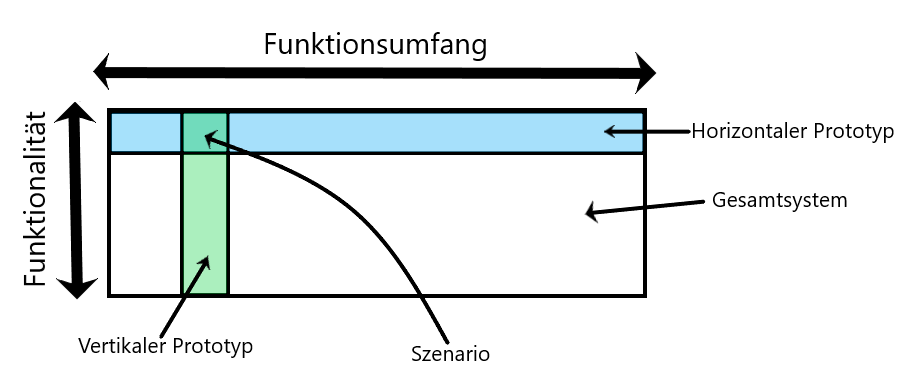
\includegraphics[width=0.8\textwidth]{resources/fundamentals/hor_ver_prototypes.png}
	\caption{Schematische Darstellung von horizontalen und vertikalen Prototypen. Quelle: In Anlehnung an \cite[S.~94]{Nielsen1994}}
	\label{img:ver_hor_protptypes}
\end{figure}

In die horizontale Dimension haben Prototypen einen breiteren Funktionsumfang beinhalten jedoch wenig bis keine Funktionalität. Horizontale Prototypen eignen sich sehr gut um ein Überblick über den Funktionsumfang des Systems zu gewinnen. Jedoch wirken Test Szenarien mit diesen Prototypen eher unrealistisch da durch die fehlende Funktionalität keine Aufgaben mit den Funktionen die der Prototyp 
bereitstellt gelöst werden können.\\
Sind Prototypen in die vertikale Richtung gestaltet, sind sie in der Funktionsumfang eingeschränkt bieten jedoch mehr Funktionalität. Diese Prototypen eignen sich sehr gut um 
besondere Aspekte eines Systems in aller Tiefe zu beleuchten. Dadurch eignen sich diese Prototypen sehr gut um bestimmte Funktionen möglichst in die Tiefe, unter realistischen 
Umständen zu testen und richtigen Aufgaben zu lösen.

Szenarien beschreibt Nielsen in \cite[S.~99]{Nielsen1994} als minimalistische Prototypen welche die Einschränkungen von horizontaler und vertikaler Prototypen vereinen. 
Nutzer können nicht mit Daten interagieren (Einschränkung horizontale Prototypen) und Nutzer können sich nicht frei im System bewegen (Einschränkung vertikaler Prototypen).
 \cite[S.~100]{Nielsen1994}Weiter definiert Nielsen, Szenarien wie folgt. 
 
 Ein Szenario beschreibt:

\begin{itemize}
	\item Einen individuellen Nutzer
	\item welcher unter bestimmten Umständen
	\item über ein bestimmtes Zeitintervall (Im Kontrast zu anderen Prototypen beinhalten Szenarien zusätzlich eine explizite Zeitdimension in welcher bestimmt wird welche Reaktion auf eine bestimmte Aktion folgt.)
	\item eine spezifischen Teil eines Computersystems nutzt
	\item um ein bestimmtes Ergebnis zu erzielen
\end{itemize}

 \cite[S.~101]{Nielsen1994} Aus Szenarien können, wenn diese ausreichend detailliert gestaltet sind für Nutzertests verwendet werden. Beispielsweise können auf Basis von Szenarien Papierprototypen erstellt werden 
 und diese von Nutzern getestet um Aufgaben zu lösen. 

\subsection{Personas}

\section{Zusammenfassung}

% AR %Objekterkennung %Situated Visualization % Was zu beachten? %Computer unterstützte Kollaboration %Usability\Engineering 
% Einleiten in Analyse: SDKs, Annotationen als Embeedded Darestellung + Zeigen und Auswählen. 



